\section{Empirical Results}\label{sec:empirical-results}
Introduction to how results are gathered with synthetic models and to the different tests implemented
%To test the algorithms presented in section~\ref{sec:flexible-resource-allocation-mechanisms}, synthetic models have
%been used to generate a list of tasks and servers. These models have been handcrafted with each attribute being
%generated from a Gaussian distribution with a mean and standard deviation.

\subsection{Evaluation of the Greedy Algorithm}\label{subsec:evaluation-of-the-greedy-algorithm}
%To compare the greedy algorithm to the optimal elastic allocation, a branch and bound was implemented to solve the
%optimisation problem in section~\ref{subsec:optimisation-problem}. In order to compare to fixed speed equivalent models,
%the minimum total resource required to run the job is found and set as the resource speeds for all of the tasks, with
%the optimal solution for running the job with the fixed speeds is found as well. To implement the greedy mechanism, the
%value density function was $\frac{v_j}{s_j + w_j + r_j}$, server selection was
%$\text{argmin}_{\forall i \in I} S^{'}_i + W^{'}_i + R^{'}_i$ and the resource allocation was
%$\min s^{'}_j + w^{'}_j + r^{'}_j$ for job $j$ and servers $I$.
%
%% Greedy mechanisms
%\begin{figure}[h]
%    \centering
%    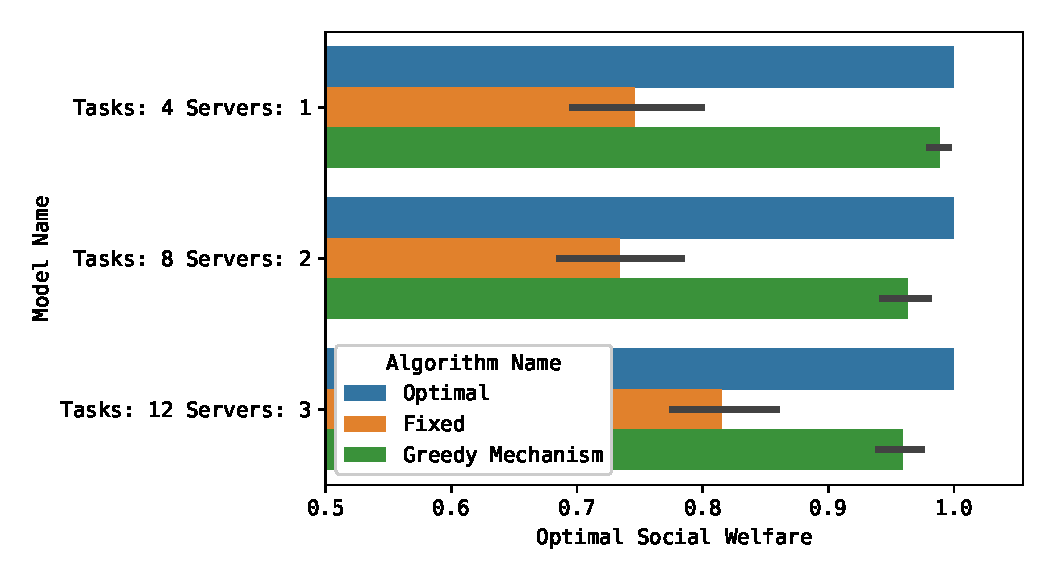
\includegraphics[width=\linewidth]{figs/empirical_evidence/greedy_mechanism}
%    \caption{Comparison of the social welfare for the greedy mechanism, optimal, relaxed problem, time limited branch and bound}
%    \label{fig:greedy-mechanism-comparison}
%\end{figure}
%As figure~\ref{fig:greedy-mechanism-comparison} shows, the greedy mechanism achieves 98\% of the optimal solution for
%the small models, the mechanism achieves within 95\% for larger models. In comparison, the fixed allocation achieves
%80\% of the optimal solution and always does worse than the social welfare of the greedy mechanism.
\subsection{Evaluation of the Auction mechanisms}\label{subsec:evaluation-of-the-auction-mechanisms}
%% Auction mechanisms
%\begin{figure}[h]
%    \centering
%    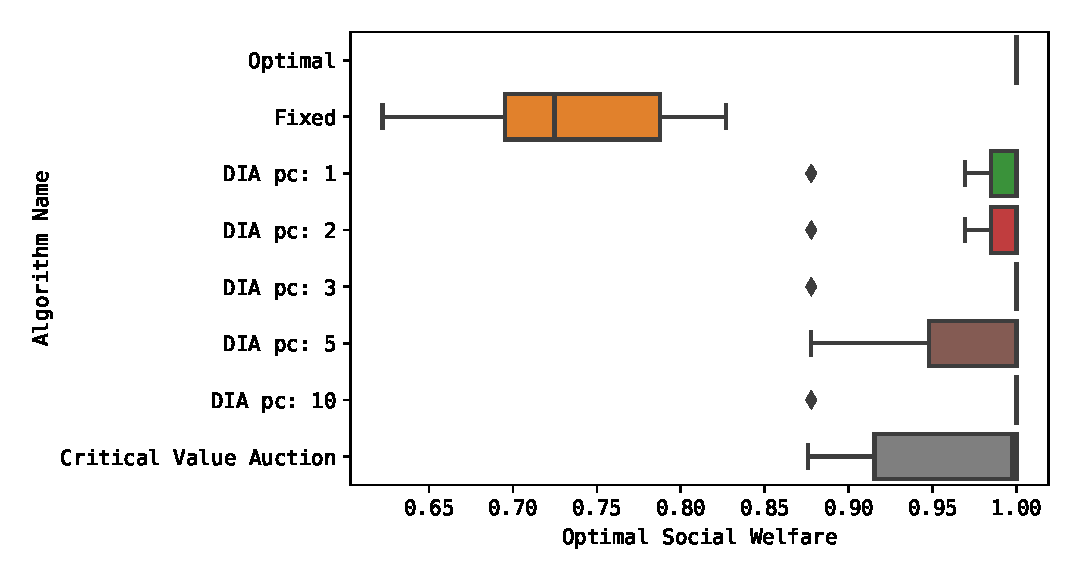
\includegraphics[width=\linewidth]{figs/empirical_evidence/auction_mechanisms}
%    \caption{Comparison of the social welfare for the auction mechanisms}
%    \label{fig:auction-mechanisms-comparison}
%\end{figure}
%Figure~\ref{fig:auction-mechanisms-comparison} compares the social welfare of the auction mechanisms: VCG auction,
%fixed resource speed VCG auction, critical value auction and the decentralised iterative auction with different price
%change variables.

\subsection{Effectiveness of Decentralised Iterative Auction Heuristics}\label{subsec:effectiveness-of-decentralised-iterative-auction-heuristics}
%% Round number
%\begin{figure}[h]
%    \centering
%    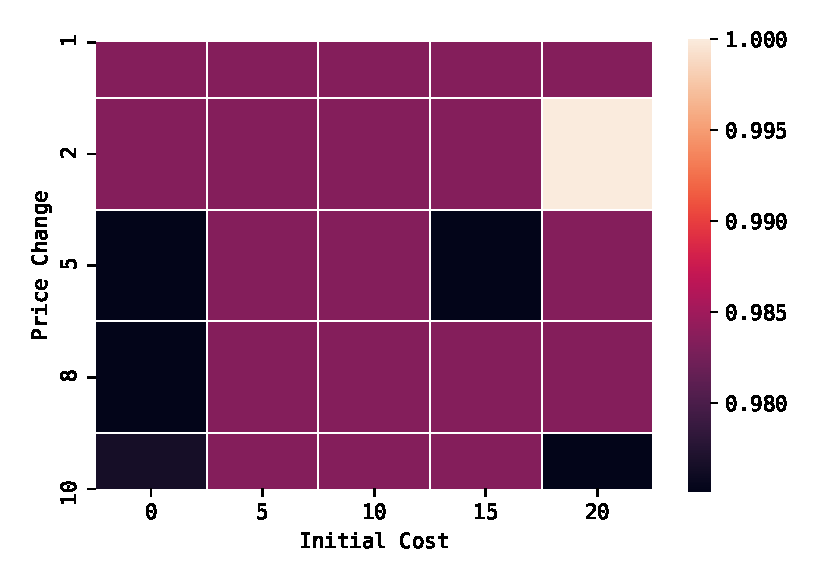
\includegraphics[width=\linewidth]{figs/empirical_evidence/iterative_round_number}
%    \caption{Average number of rounds with a price change variables and task initial cost}
%    \label{fig:iterative-round-number}
%\end{figure}
%\begin{figure}[h]
%    \centering
%    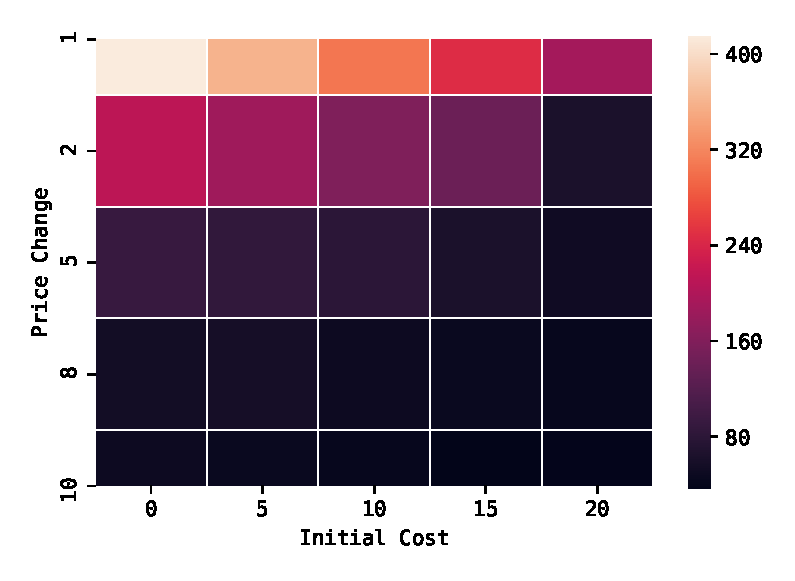
\includegraphics[width=\linewidth]{figs/empirical_evidence/iterative_social_welfare}
%    \caption{Average social welfare with a price change variables and task initial cost}
%    \label{fig:iterative-social-welfare}
%\end{figure}
%Within the context of edge cloud computing, the number of rounds for the decentralised iterative auction is important
%to making it a feasible auction as it is proportional to the time required to run. We investigated the effect of two
%heuristic on the number of rounds and social welfare of the auction; the price change variable and initial cost
%heuristic. With an auction using as minimum heuristic values for the price change and initial cost,
%figure~\ref{fig:iterative-round-number}, on average 400 rounds were required for the price to converge while an auction
%using a price change of 10 and initial cost of 20 means that only on average 80 rounds are required, 5x less. But by
%using high initial cost and price change heuristics, this can prevent tasks from being allocated,
%figure~\ref{fig:iterative-social-welfare}, shows that the difference in social welfare is only 2\% from minimum to
%maximum heuristics.

\subsection{Possibility of Task Mutation in Decentralised Iterative Auction}\label{subsec:possibility-of-task-mutation-in-decentralised-iterative-auction}
%Mutation auction
%\begin{figure}
%    \centering
%    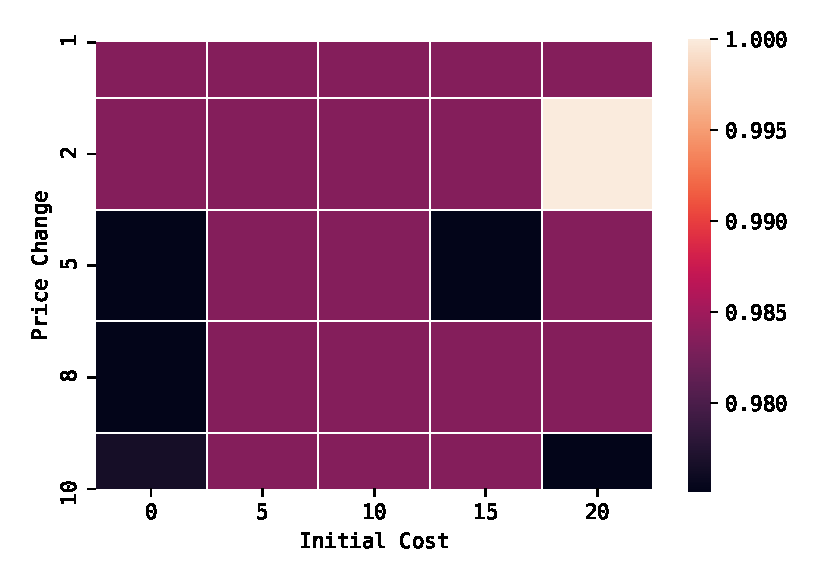
\includegraphics[width=\linewidth]{figs/empirical_evidence/iterative_round_number}  %% TODO update with the mutated png
%    \caption{Difference in task price to a truthful task and misreported task}
%    \label{fig:auction-mutation}
%\end{figure}
%As the decentralised iterative auction presented in section~\ref{subsec:decentralised-iterative-auction} is not
%incentive compatible, it is possible that misreporting of task attribute can decrease the price paid by a task.
%Figure~\ref{fig:auction-mutation} is a scatter graph of the a task (in orange) and the price of a misreported task
%(in blue). Misreported task were generated by increase the task resource requirements or by decreasing the task value
%or deadline that would substituted for the original truthful task. As the figure clearly shows, in almost all cases of
%mutation causes the

\subsection{Effect of Server Resource Capacity Ratio}\label{subsec:affect-of-server-resource-capacity-ratio}

\subsection{Batching verse Online task allocation}\label{subsec:batching-verse-online-task-allocation}
